\documentclass[a4paper,12pt]{article}
\usepackage{graphicx}
\usepackage{hyperref}
\usepackage{titlesec}
\usepackage{booktabs}
\usepackage{float}
\usepackage{xcolor}
\usepackage{mathptmx}  % Times New Roman-like font
\usepackage{amsmath} 

\title{\textbf{Speech Understanding}\\
\bigskip
\bigskip
\bigskip
{Programming Assignment-1}\\
\bigskip\bigskip\bigskip
{Project Report - Q-1} 
\bigskip\bigskip\bigskip\\
    {Speech Emotion Recognition (SER)}
}


\author{\textbf{Prepared By:}\\Om Prakash Solanki (M23CSA521)\\Shyam Vyas (M23CSA545)}

\begin{document}
\maketitle
\newpage
\section{Abstract}
Speech Emotion Recognition (SER) enhances Human-Computer Interaction (HCI) by allowing machines to interpret emotions from speech. This capability is crucial for improving user experience in applications such as virtual assistants, mental health monitoring, and customer service. Traditional SER methods struggle with limited labeled datasets, restricting their effectiveness. Self-supervised learning addresses this issue by leveraging large, unlabeled speech datasets.\\
This study evaluates two self-supervised learning models, Wav2Vec 2.0 and Whisper-large-v3, within an end-to-end SER framework. Our analysis compares their accuracy and generalization abilities. The findings indicate that while both models perform well, firdhokk’s model achieves higher accuracy and better generalization in English-centric datasets. However, it is unclear whether this advantage arises from model architecture or differences in pre-training data. Future research should control for these variables to ensure fair comparisons and optimize SER performance.
\newpage
\tableofcontents
\newpage

\section{Introduction}
\subsection{Introduction}
Speech Emotion Recognition (SER) enables machines to analyze and interpret emotional cues in speech, enhancing various real-world applications. As a subset of affective computing, SER plays a vital role in personalizing user interactions across domains such as healthcare, entertainment, and customer support. Conventional SER approaches rely on labeled datasets, which are often scarce and expensive to annotate, limiting their effectiveness in real-world scenarios.

To overcome these challenges, recent research has turned to self-supervised learning, which leverages large volumes of unlabeled speech data for feature extraction. This study investigates two leading models, Wav2Vec 2.0 and Whisper-Large-V3, utilizing a modular Upstream + Downstream framework. By evaluating these models’ capabilities, we aim to enhance SER systems' robustness and reliability across diverse linguistic settings.

\subsection{Scope}
This project focuses on building and evaluating a Speech Emotion Recognition (SER) system based on deep learning methodologies. The primary objective is to classify emotions such as happiness, sadness, anger, and neutrality from speech recordings using advanced machine learning models.\\
The research specifically examines the performance of Whisper-Large-V3 and Wav2Vec 2.0, determining their effectiveness in emotion recognition tasks. By integrating state-of-the-art self-supervised learning models, the project aims to enhance the accuracy and generalization of SER systems. The findings will contribute to improved speech-based applications, including interactive AI systems, emotion-aware chatbots, and automated mental health diagnostics.

\newpage

\section{Background}
\subsection{Speech Emotion Recognition}
Speech emotion recognition (SER) is a computational technique that identifies human emotions from spoken utterances. The field has garnered significant interest over the past decades, particularly in applications such as human computer interaction (HCI) systems and psychological treatments. This technology aims to discern the emotional state of a speaker using various acoustic features of speech which are largely consistent across languages, making SER adaptable to different linguistic contexts.

One of the most established databases in this field is the Interactive Emotional Dyadic Motion Capture database (IEMOCAP) which provides a standard benchmark for SER studies. Initial methods in SER utilized combinations of convolutional neural networks (CNNs) and long short-term memory (LSTM) networks to process and learn from audio data. However, recent advances have seen the rise of attention-based models which excel at focusing on relevant aspects of the audio input, thereby enhancing recognition accuracy. Furthermore, the advent of self-supervised learning models has transformed the landscape of SER by leveraging unlabeled data to achieve state-of-the-art results in emotion detection, as demonstrated by Yang et al.

The appeal of speech as a modality for emotion recognition lies in its accessibility and reliability; it is less susceptible to physical obstructions or variations such as facial occlusions or differences in physical gestures. Additionally, SER systems are integral to enhancing the quality of various service applications, from interactive media and e-tutoring to customer service and surveillance. These systems not only facilitate better user interactions by adjusting responses based on emotional cues but also support dynamic content adaptation in online platforms.

Despite its versatility, SER faces significant challenges, particularly in real-life applications where the accuracy of emotion recognition remains suboptimal. The primary impediment is the environmental variation in speaker characteristics, language, and cultural context between the training and deployment stages of SER systems. This mismatch often leads to decreased performance when the systems are applied in natural settings. To address these discrepancies, research has increasingly focused on creating models that are independent of the speaker, text, and language. These strategies include cross-corpus studies which inherently handle variations in speaker identity, textual content, and linguistic properties.

\subsection{Self-supervised learning}
In the evolving field of machine learning, Self-Supervised Learning (SSL) has emerged as a significant paradigm shift. SSL offers a robust alternative to traditional supervised and unsupervised learning methods. Unlike supervised learning, which relies on manually annotated data, SSL utilizes unlabeled data—thus circumventing the labor-intensive process of labeling, which can be both time-consuming and costly. This technique automates the generation of labels within the data, exploiting inherent relationships and patterns which simplifies the learning process without human intervention.

The origin of SSL can be traced back to robotics, where it was first utilized to assign labels automatically to training data. The primary mechanism of SSL involves providing a neural network, such as a Convolutional Neural Network (ConvNet), input data where certain parts of the input are obscured. The model is then trained to predict these hidden parts from the visible segments of the data. This approach mimics the natural learning process observed in infants, who learn about their environment through exploration and interaction without direct supervision. The surroundings of an infant thus provide indirect supervision that facilitates learning. SSL is distinct from unsupervised learning because it still uses labels, but these are generated automatically by the system rather than manually annotated by humans. This method employs two principal strategies: auxiliary pretext tasks and contrastive learning. Pretext tasks involve creating pseudo-labels by harnessing attributes of the dataset to perform tasks such as image completion, grayscale conversion, and predicting obscured segments of images. These tasks generate representations that are instrumental in training the model.

Contrastive learning, on the other hand, focuses on distinguishing between different augmentations or perspectives of the same image. By recognizing the variations between these views, the model enhances its understanding and feature extraction capabilities. This method is particularly effective in learning detailed and nuanced representations that are useful for complex vision tasks such as classification, segmentation, and object detection.

The concept of SSL is not confined to computer vision but has also been significantly applied in the field of natural language processing (NLP). Techniques like Bidirectional Encoder Representations from Transformers (BERT) utilize SSL for various NLP tasks including neighbor sentence prediction and auto-regressive language modeling, which help in understanding and generating language-based data.

\subsection{Convolutional Neural Networks}
Convolutional Neural Networks (CNNs) are a class of deep neural networks highly effective in areas such as image recognition, speech recognition, and natural language processing. Rooted in the study of the animal visual cortex, the CNN architecture is inspired by the pattern recognition and signal processing that occurs in the human brain. The foundational work in CNNs began with discoveries in the visual systems of animals, leading to the initial artificial models in the 1980s and 1990s by Fukushima (1980) and LeCun et al. (1990), respectively, who developed the early neural network models that could recognize visual patterns such as handwritten digits from pixel images.

CNNs consist primarily of three types of layers as illustrated in Figure \ref{fig:cnn_architecture}: convolutional layers, pooling layers, and fully connected layers - each serving a distinct purpose:
\begin{itemize}
    \item \textbf{Convolutional layers:} These layers perform the convolution operation that filters the input to extract features. The filters applied across the input not only detect features such as edges but also preserve the relationship between pixels by learning image features using small squares of input data.
    \item \textbf{Pooling layers:} Sometimes referred to as downsampling, pooling reduces the dimensionality of each feature map while retaining the most essential information. Max pooling and average pooling are the two commonly used techniques in this layer.
    \item \textbf{Fully connected layers:} These layers connect every neuron in one layer to every neuron in the next layer, which is typical in traditional neural networks. It is in these layers where the classification process occurs, based on the features analyzed in the convolutional and pooling layers.
\end{itemize}

\begin{figure}[H]
    \centering
    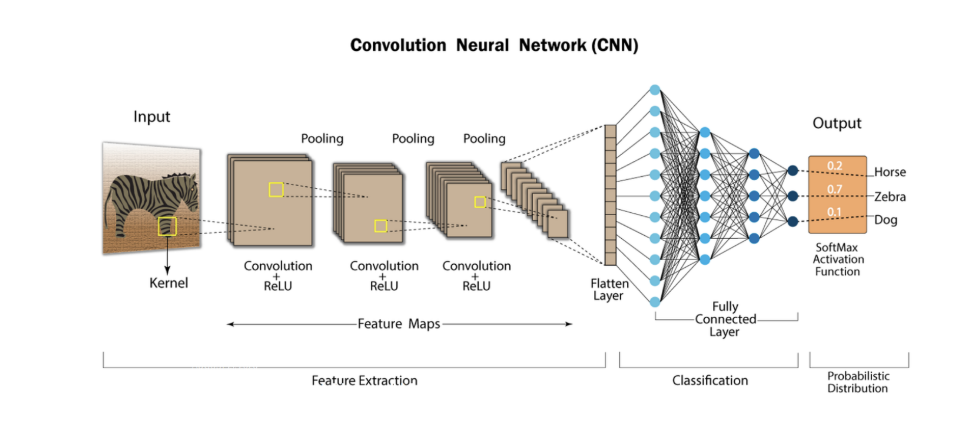
\includegraphics[width=1\textwidth]{TestImage.png}
    \caption{CNN Architecture}
    \label{fig:cnn_architecture}
\end{figure}

The functioning of a CNN involves the processing of an input through multiple convolutional and pooling layers that extract various features. The output of these layers is then flattened and fed into fully connected layers for classification purposes. The backpropagation algorithm is commonly used for training CNNs, utilizing gradient descent to update the network weights. Furthermore, each layer within a CNN transforms activations to another through a differentiable function. These transformations include (1) ReLU activation function and (2) Local connectivity and shared weights.

\subsection{Transformers}
The emergence of the Transformer model in natural language processing (NLP) marks a significant shift from traditional architectures like recurrent neural networks (RNNs) and long short-term memory (LSTM) networks. Before the emergence of Transformers, RNNs were often used due to their ability to process sequences of data. This was done by passing the output of one neuron into the input of another, thus mimicking a form of memory useful for tasks such as machine translation and predictive text generation. However, RNNs faced significant challenges, such as the vanishing gradient problem, which made training over long sequences difficult.

To address these limitations, LSTM networks were introduced by Hochreiter and Schmidhuber in 1997, which were better at handling longer data sequences but still suffered from performance degradation as the sequence length increased. Additionally, the sequential nature of RNNs and LSTMs limited their ability to be parallelized, making the training process time-consuming and computationally expensive.

The introduction of attention mechanisms by researchers such as in marked a pivotal development. These attention mechanisms allowed models to focus on specific, relevant parts of the input data, improving the model’s performance on longer sequences by encoding the input into multiple ‘memory’ vectors rather than a single fixed-length vector. This allowed for selective attention to different parts of the input during the prediction phase, which was a significant improvement over the traditional encoder-decoder structure of RNNs and LSTMs.

Building on this concept of attention, Vaswani et al. introduced the Transformer architecture, which completely abstains from recurrent units in favor of an architecture based solely on attention mechanisms. This architecture uses what is known as ‘Multi-head Attention’ to process different segments of the input data in parallel, significantly enhancing the efficiency and speed of training by leveraging the parallel computational capabilities of modern hardware. This design not only allowed for the handling of longer sequences without degradation in performance but also reduced training times considerably when large datasets and computing resources were available.

\subsubsection{Transformer Model Architecture}
The Transformer model, is designed entirely around an attention mechanism, eliminating the need for recurrence. It consists of an encoder-decoder structure shown in Figure \ref{fig:transformer_architecture}, where both parts use stacked self-attention and fully connected layers.

\begin{figure}[H]
    \centering
    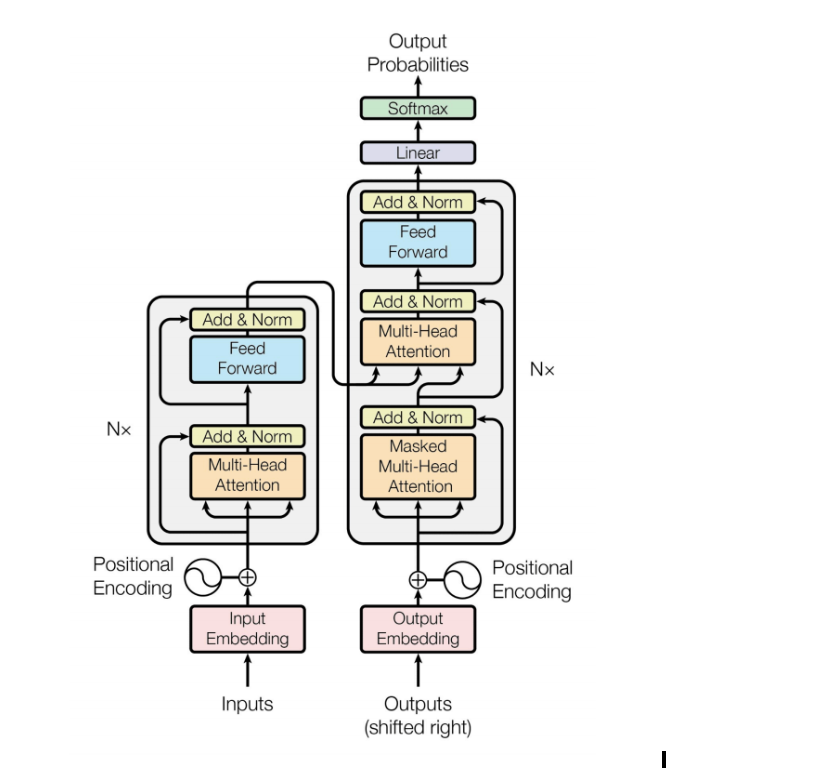
\includegraphics[width=0.6\textwidth]{transformer_architecture.png}
    \caption{The Transformer Model Architecture }
    \label{fig:transformer_architecture}
\end{figure}

{Encoder and Decoder Stacks}
{Encoder}
The encoder is composed of a stack of $N = 6$ identical layers. Each layer has two sub-layers: a multi-head self-attention mechanism and a position-wise fully connected feed-forward network. A residual connection is employed around each of the sub-layers, followed by layer normalization:
\begin{equation}
\[
\text{LayerNorm}(x + \text{Sublayer}(x))
\
\end{equation}
where \(x\) is the input to each sub-layer and \(\text{Sublayer}(x)\) is the function implemented by the sub-layer itself.

{Decoder}
The decoder also consists of $N = 6$ identical layers. In addition to the two sub-layers present in the encoder, the decoder has a third sub-layer that performs multi-head attention over the output of the encoder stack. This is to prevent positions from attending to subsequent positions, ensuring that the predictions for position \(i\) can depend only on the known outputs at positions less than \(i\).

{Attention Mechanism}
{Scaled Dot-Product Attention}
The attention function computes the dot products of the query with all keys, divides each by \(\sqrt{d_k}\), and applies a softmax function to obtain the weights on the values:
\begin{equation}
\[\left
\text{Attention}(Q, K, V) = \text{softmax}\left(\frac{QK^T}{\sqrt{d_k}}\right)V
\]\right
\end{equation}\\
where \(Q\), \(K\), and \(V\) are matrices representing queries, keys, and values, respectively.

{Multi-Head Attention}
Instead of performing a single attention function, it is beneficial to linearly project the queries, keys, and values \(h\) times with different, learned linear projections to \(d_k\), \(d_k\), and \(d_v\) dimensions, respectively. Then, the attention function is performed in parallel, yielding \(d_v\)-dimensional output values. These are concatenated and once again projected, resulting in the final values:
\begin{equation}
\left
\text{MultiHead}(Q, K, V) = \text{Concat}(\text{head}_1, \dots, \text{head}_h) W_O
\right
\end{equation}\\
where each \(\text{head}_i\) is defined as:
\begin{equation}
\left
\[
\text{head}_i = \text{Attention}(Q W_i^Q, K W_i^K, V W_i^V)
\]
\right
\end{equation}\\
and the projections are parameter matrices \(W_i^Q \in \mathbb{R}^{d_{\text{model}} \times d_k}\), \(W_i^K \in \mathbb{R}^{d_{\text{model}} \times d_k}\), \(W_i^V \in \mathbb{R}^{d_{\text{model}} \times d_v}\), and \(W_O \in \mathbb{R}^{h d_v \times d_{\text{model}}}\).

{Position-wise Feed-Forward Networks}
Each layer of the encoder and decoder contains a fully connected feed-forward network, which is applied to each position separately and identically:
\begin{equation}
\left
\[
\text{FFN}(x) = \max(0, x W_1 + b_1) W_2 + b_2
\]
\right
\end{equation}\\
where \(W_1\), \(W_2\) are weight matrices and \(b_1\), \(b_2\) are bias vectors.

{Positional Encoding}\\

Since the model contains no recurrence and no convolution, positional encodings
are added to the input embeddings at the bottoms of the encoder and decoder
stacks:

\begin{equation}
    PE(pos, 2i) = \sin \left( \frac{pos}{10000^{\frac{2i}{d_{model}}}} \right)
\end{equation}

\begin{equation}
    PE(pos, 2i + 1) = \cos \left( \frac{pos}{10000^{\frac{2i}{d_{model}}}} \right)
\end{equation}

\subsection{Wav2Vec 2.0}

Wav2Vec 2.0, developed by Meta AI, is a state-of-the-art speech processing model that leverages the transformer architecture to generate highly effective contextualized representations from raw audio signals. The core of Wav2Vec 2.0’s architecture consists of three primary modules illustrated in Figure \ref{fig:architecture_Wav2Vec2}: a feature encoder, a transformer module, and a quantization module .

\begin{figure}[H]
    \centering
    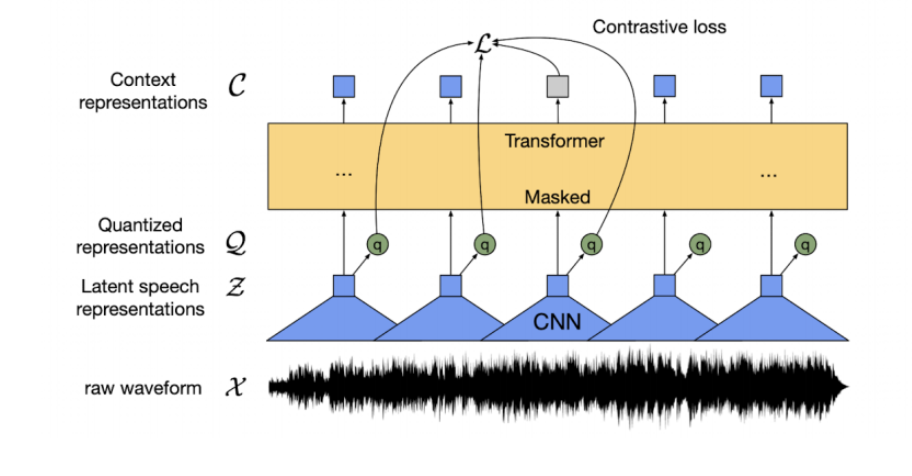
\includegraphics[width=0.5\linewidth]{architecture_Wav2Vec2.png}
    \caption{Architecture of Wav2Vec 2.0}
    \label{fig:architecture_Wav2Vec2}
\end{figure}

The feature encoder is a multi-layer convolutional neural network (CNN) that processes the input raw waveform into latent speech representations. These features are partially masked and fed into the transformer module, which enhances them into high-level, contextualized representations. Subsequently, the quantization module then discretizes these features into a series of discrete embeddings, forming a trainable codebook, which are used as targets for model training.

The training of Wav2Vec 2.0 utilizes a self-supervised setting akin to masked language modeling techniques used in BERT. It involves predicting the quantized representations of masked audio segments based on their unmasked context. Specifically, the model masks contiguous time steps from the CNN encoder’s outputs and attempts to predict the quantized version of these masked features at the transformer’s output. 

The objective function used during this phase is a contrastive loss, where the similarity between the contextual encoder outputs and the quantized CNN encoder representations is maximized against a set of distractor samples drawn from the same utterance. The objective function during training is defined as follows:

\begin{figure}[H]
    \centering
    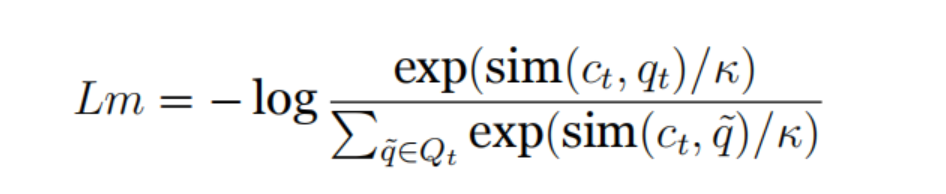
\includegraphics[width=0.5\linewidth]{Lostfunction.png}
\end{figure}

where \(\text{sim}(a, b) = \frac{a^T b}{\|a\| \|b\|}\) denotes the cosine similarity, \(c_t\) represents the contextualized encoder output at time step \(t\), \(q_t\) is the quantized representation of the encoder output, \(Q_t\) is the set including \(q_t\) and \(K = 100\) distractors sampled from other masked time steps within the same utterance, and \(\kappa = 0.1\) is a temperature parameter. The contrastive loss is augmented by \(L2\) regularization and a diversity loss, which helps in effectively utilizing the quantized codebook representations.

Further enhancing its utility, Wav2Vec 2.0 can be fine-tuned for various speech-related tasks such as automatic speech recognition (ASR) as demonstrated in \cite{ref23}. The fine-tuning involves adding a randomly initialized linear projection to the contextual encoder’s output and optimizing the Connectionist Temporal Classification (CTC) loss to improve performance specifically on ASR tasks. This fine-tuning process has shown significant improvements in ASR accuracy.

\subsection{Whisper-Large-V3}
Whisper-Large-V3 is an advanced automatic speech recognition (ASR) model developed by OpenAI. It is designed to process speech with high accuracy, leveraging deep learning techniques and large-scale training datasets. Whisper models are known for their ability to transcribe multilingual speech, perform speech-to-text conversion, and capture nuanced acoustic features that can be useful for tasks like Speech Emotion Recognition (SER). 

Whisper-Large-V3 benefits from extensive pretraining on diverse audio datasets, making it robust in handling variations in tone, pitch, and speech patterns.

\subsection{Related work}

There exist previous studies that have significantly contributed to the field of speech emotion recognition (SER). One such notable work is by Morais et al., who developed a modular end-to-end SER system that utilizes self-supervised pre-trained features. This system is particularly innovative due to its use of an Upstream + Downstream architecture, which allows for the easy integration of a variety of self-supervised features.

The authors employed advanced self-supervised models, specifically Wav2Vec 2.0 and HuBERT, known for their effective speech representation capabilities. These models form the backbone of the upstream component of their system, which is critical for extracting robust features from speech data. The downstream component then classifies these features into categorical emotion states using data from the IEMOCAP dataset.

Their findings demonstrate that the proposed system, despite using only the speech modality, achieves state-of-the-art results comparable to those of multimodal systems that also include text. This is particularly significant for scenarios where only speech data is available, such as in call center analytics. 

Morais et al.’s study not only highlights the effectiveness of self-supervised learning models in improving SER systems but also opens up avenues for future research. They suggest that extending the system to support multitask learning and incorporating additional modalities such as text and visuals could further enhance its capabilities.

Following the innovative approach by Morais et al., another significant advancement in the field of speech emotion recognition (SER) is presented by Yingzhi Wang and colleagues from Zaion Lab in Paris, France. Their study, focusing on the fine-tuning of self-supervised models such as Wav2Vec 2.0 and HuBERT, expands the utility of these models beyond their traditional application in Automatic Speech Recognition (ASR) to include Speech Emotion Recognition (SER), Speaker Verification (SV), and Spoken Language Understanding (SLU).

Wang et al. explore both partial and entire fine-tuning methods on these pre-trained models—demonstrating a nuanced approach to enhancing model performance across various speech tasks. Specifically for SER, their experiments on the IEMOCAP dataset resulted in substantial improvements, with the models achieving up to 79.58\% weighted accuracy in speaker-dependent settings and 73.01\% in speaker-independent settings. These results underscore the potential of fine-tuned self-supervised models in capturing and classifying complex emotional states from speech data.

\newpage
\section{Method}
\subsection{Dataset}

\subsubsection{Toronto Emotional Speech Set -}
For our study on Speech Emotion Recognition (SER), we utilize the Toronto Emotional Speech Set (TESS) dataset, available at link. TESS is a publicly available dataset designed to study emotional speech variations in older and younger female speakers. It consists of 2,800 speech samples recorded by two actresses, portraying seven emotions: anger, disgust, fear, happiness, pleasant surprise, sadness, and neutral.\\
Each sentence in the dataset was spoken in a neutral tone and then re-recorded in an emotionally expressive manner. The dataset is widely used in speech processing research due to its high-quality recordings and well-annotated labels, making it an ideal choice for training and evaluating Speech Emotion Recognition (SER) models. This publicly available dataset is well-regarded in the research community for its diverse and well-annotated audio-visual recordings of emotional expressions.

\paragraph{Data Processing}
The TESS dataset serves as the primary data source for this study on Speech Emotion Recognition. Despite its high-quality recordings, the audio files in TESS are not natively sampled at the 16 kHz rate required by the pre-trained models. Thus, to align the TESS dataset with the input requirements of our models, it was necessary to downsample the audio files from their original sample rates to 16 kHz.

\subsubsection{Surrey Audio-Visual Expressed Emotion (SAVEE) -}

For our study on Speech Emotion Recognition (SER), we utilize the Surrey Audio-Visual Expressed Emotion (SAVEE) dataset, available at \href{https://www.kaggle.com/datasets/ejlok1/surrey-audiovisual-expressed-emotion-savee}{link}. SAVEE is a publicly available dataset designed to analyze emotional speech variations in male speakers. It consists of 480 utterances recorded by four native English-speaking male actors, portraying seven emotions: anger, disgust, fear, happiness, sadness, surprise, and neutral.

Each sentence in the dataset was initially spoken in a neutral tone and then re-recorded with emotional expressions. The dataset is widely used in speech and audio processing research due to its high-quality recordings and well-defined emotional labels, making it a valuable resource for training and evaluating Speech Emotion Recognition (SER) models. SAVEE is recognized in the research community for its diverse emotional expressions and well-structured annotations, making it an essential dataset for studying emotional variations in speech.


\paragraph{Data Processing}
The SAVEE dataset serves as a key data source for this study on Speech Emotion Recognition. While the dataset provides high-quality recordings, the audio files in SAVEE are originally sampled at 44.1 kHz. To ensure compatibility with the input requirements of our pre-trained models, it was necessary to downsample the audio files to 16 kHz. This preprocessing step standardizes the dataset, allowing for consistent feature extraction and model training.

\subsection{Implementation and Tools}
To evaluate our Speech Emotion Recognition (SER) models, we employed a suite of powerful tools and frameworks that are widely recognized for their robustness and versatility in machine learning and deep learning tasks.

\begin{itemize}
    \item \textbf{Hugging Face Transformers}: The Hugging Face Transformers library was utilized to integrate state-of-the-art natural language processing models into our SER pipeline. This library provided pre-trained transformer checkpoints for Wav2Vec2.0 and Whisper-Large-V3, enabling seamless model loading, configuration, and fine-tuning. By leveraging Hugging Face, we streamlined the deployment of these advanced models for emotion recognition from speech data.
    
    \item \textbf{PyTorch}: As the core deep learning framework, PyTorch facilitated the implementation and optimization of our SER models. Its dynamic computational graph and modular design made it an ideal choice for deep learning research. PyTorch's compatibility with GPU acceleration allowed for efficient training and fine-tuning of model parameters, significantly improving processing speed and scalability.
    
    \item \textbf{scikit-learn}: To support model training and evaluation, we employed scikit-learn, a widely used machine learning library. This toolkit was instrumental in preprocessing data, splitting datasets, and implementing classification algorithms. Furthermore, it provided essential evaluation metrics such as accuracy, precision, recall, and F1-score to assess model performance comprehensively.
    
    \item \textbf{Weights \& Biases}: Experiment tracking and performance monitoring were managed using Weights \& Biases. This tool enabled real-time logging of training progress, visualization of model performance trends, and hyperparameter optimization. By integrating Weights \& Biases, we ensured reproducibility and facilitated efficient model comparison throughout the development process.
\end{itemize}

\subsection{Pretrained Models}
\subsubsection{wav2vec2-large-xlsr-53}
We employed the pretrained model \texttt{facebook/wav2vec2-large-xlsr-53} for the Wav2Vec 2.0 architecture. The XLSR-53 model is an extension of Wav2Vec 2.0, designed to learn cross-lingual speech representations by pretraining on raw waveform data from multiple languages. Fine-tuned on labeled data, XLSR-53 demonstrates significant improvements in cross-lingual pretraining over monolingual approaches. On benchmarks such as CommonVoice, it achieved a 72\% relative reduction in phoneme error rate and a 16\% improvement in word error rate on the BABEL dataset compared to previous models. The XLSR-53 model is fine-tuned using the Common Voice dataset, which comprises over 9,283 recorded hours across 60 languages, providing a robust foundation for multilingual speech recognition.

\subsubsection{Whisper-Large-V3}
We employed the pretrained model \texttt{Whisper-Large-V3}, developed by OpenAI, for automatic speech recognition and emotion classification. Whisper-Large-V3 is a transformer-based model trained on a massive multilingual dataset, making it robust for speech recognition across different languages and dialects. It leverages a combination of supervised fine-tuning and self-supervised learning, allowing it to capture intricate speech characteristics. Due to its high accuracy in speech recognition, Whisper-Large-V3 is well-suited for SER applications, where subtle emotional nuances in voice need to be effectively classified.

\subsubsection{Rationale for Model Selection}
The selection of the two models was guided by several factors:
\begin{itemize}
    \item \textbf{Pretraining on ASR Tasks}: Both models have been fine-tuned for automatic speech recognition (ASR), which typically yields better performance in downstream speech-related tasks like speech emotion recognition (SER). Their pretraining allows them to extract nuanced features essential for recognizing emotional cues in speech.
    \item \textbf{Popularity and Credibility}: These models are among the most popular for their respective architectures on the Hugging Face model hub, which speaks to their reliability and widespread validation by the community.
    \item \textbf{Ease of Implementation}: Both checkpoints are well-documented and supported, facilitating straightforward integration and implementation in our system compared to other available models on the platform.
\end{itemize}

\subsection{Evaluation}
The classifiers are tested on a set of data that has not been previously seen during training (the testing set). This evaluation reflects the model’s ability to generalize to new, unseen data. For our study, we utilize an $7 \times 7$ confusion matrix suitable for multiclass classification with seven labels. Each class is considered as the positive class against all other classes, which are combined as the negative class for each calculation iteration.

The structure of a general $n \times n$ confusion matrix is:
\begin{itemize}
    \item The rows represent the actual classes.
    \item The columns represent the predicted classes.
\end{itemize}

\begin{figure}[H]
    \centering
    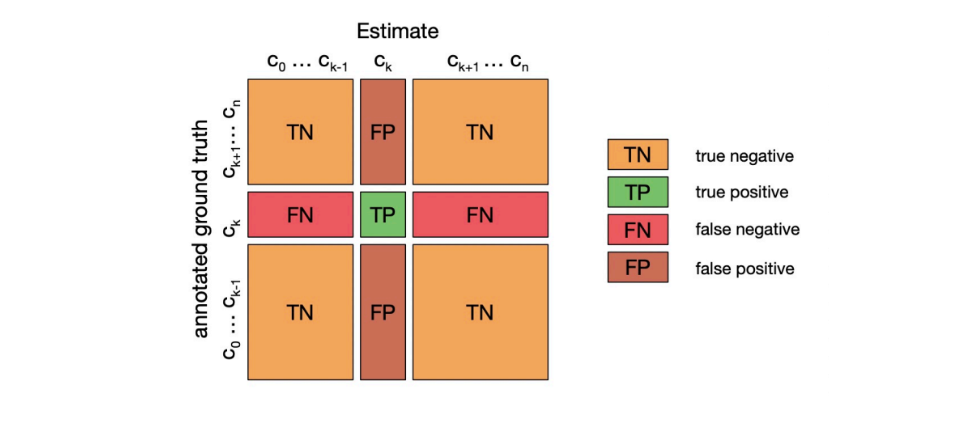
\includegraphics[width=1\linewidth]{confusion_matrix.png}
\end{figure}

Figure 3.6: The structure of a confusion matrix for the classification of n classes, where the true positive (TP), true negatives (TN), false positives (FP), and false negatives (FN) are highlighted for class number k.\\


Utilizing the Confusion Matrix, we can retrieve several critical metrics for evaluation; Accuracy, Precision, Recall, and F1-Score. Accuracy measures the overall correctness of the model and is defined as the ratio of correctly predicted observations to the total observations. It can be mathematically represented as:
\begin{figure}[H]
    \centering
    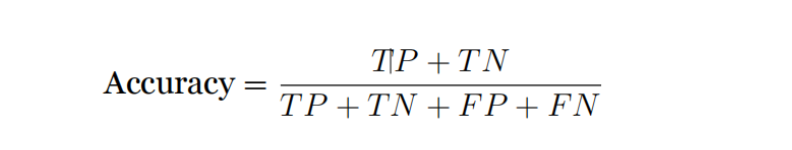
\includegraphics[width=.8\linewidth]{accuracy.png}
\end{figure}

To continue, Precision for a class measures the accuracy of positive predictions. It is calculated as the ratio of correctly predicted positive observations to the total predicted positive observations for that class:
\begin{figure}[H]
    \centering
    
\includegraphics[width=1\linewidth]{Precision.png}
\end{figure}

Subsequently, Recall, or Sensitivity, measures the model’s ability to identify all relevant instances within a dataset. For a given class, it is the ratio of correctly predicted positive observations to all observations in the actual class:
\begin{figure}[H]
    \centering
    
\includegraphics[width=.6\linewidth]{Recall.png}
\end{figure}


Lastly, The F1-score is the harmonic mean of Precision and Recall. It takes both false positives and false negatives into account and is defined as:

\begin{figure}[H]
    \centering
    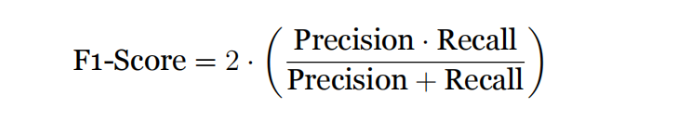
\includegraphics[width=0.7\linewidth]{F1Score.png}
\end{figure}
We compare the calculated metrics (Accuracy, Precision, Recall, and F1-Score) for both Wav2Vec 2.0 and Whipser-Large-V3 based on their performance on the testing dataset. This comparison aims to elucidate the strengths and weaknesses of each model across different emotional classes, providing insights into their applicability in practical scenarios.


\newpage
\section{Results}
\subsection{Performance of the Whisper-Large-V3 Model - With TESS Dataset}
\subsubsection{Final Evaluation Results}
\begin{figure}[H]
    \centering
    
\includegraphics[width=1\linewidth]{FinalResults1.png}
    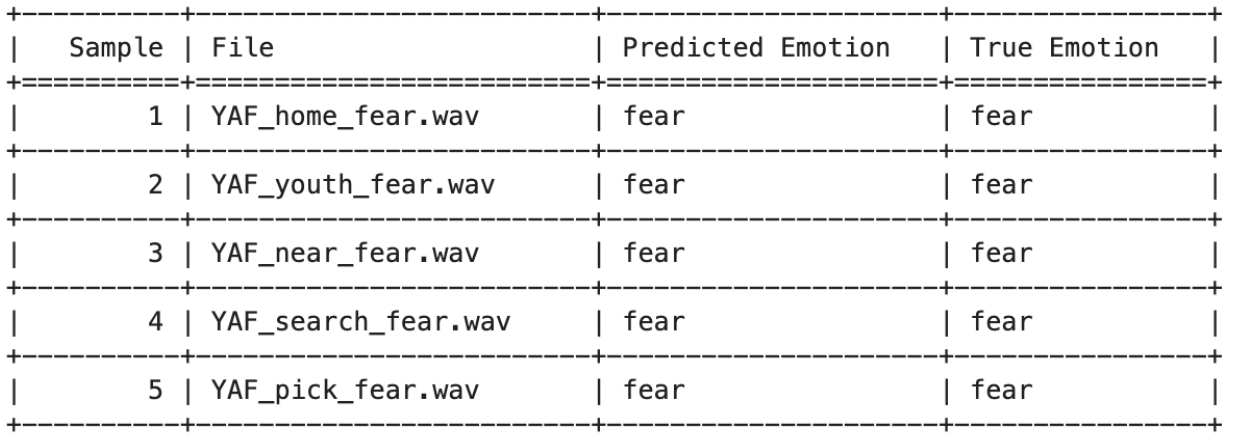
\includegraphics[width=1\linewidth]{FinalResults2.png}
\end{figure}
\begin{figure}[H]
    \centering
    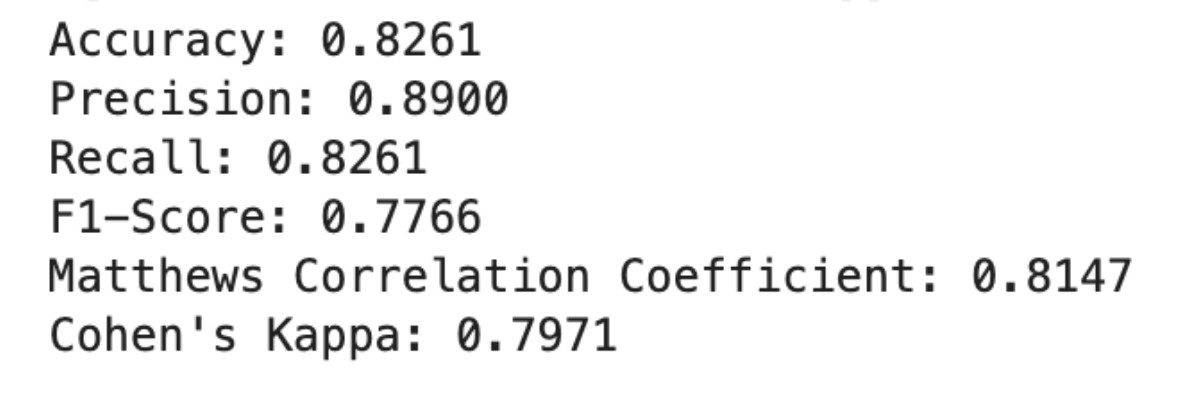
\includegraphics[width=1\linewidth]{FinalResults3.png}
\end{figure}
\subsubsection{Classification Report}
\begin{figure}[H]
    \centering
    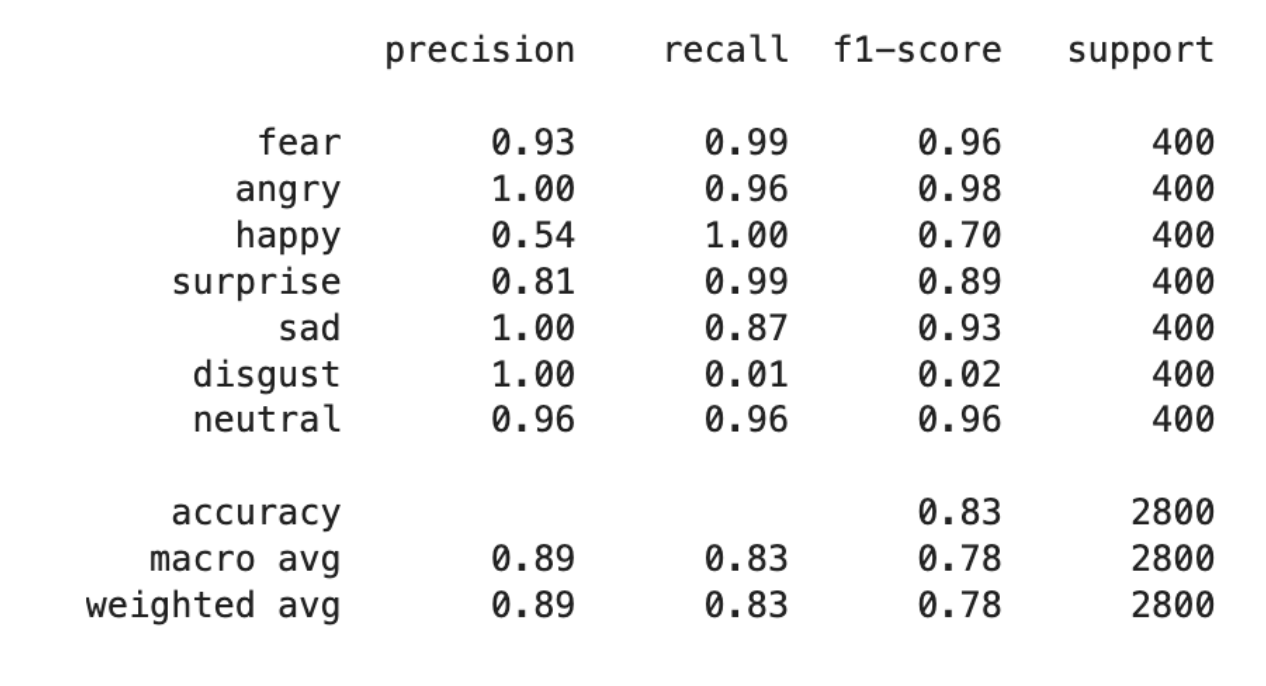
\includegraphics[width=1\linewidth]{FinalResults5.png}
\end{figure}
\subsubsection{Confusion Matrix}
\begin{figure}[H]
    \centering
    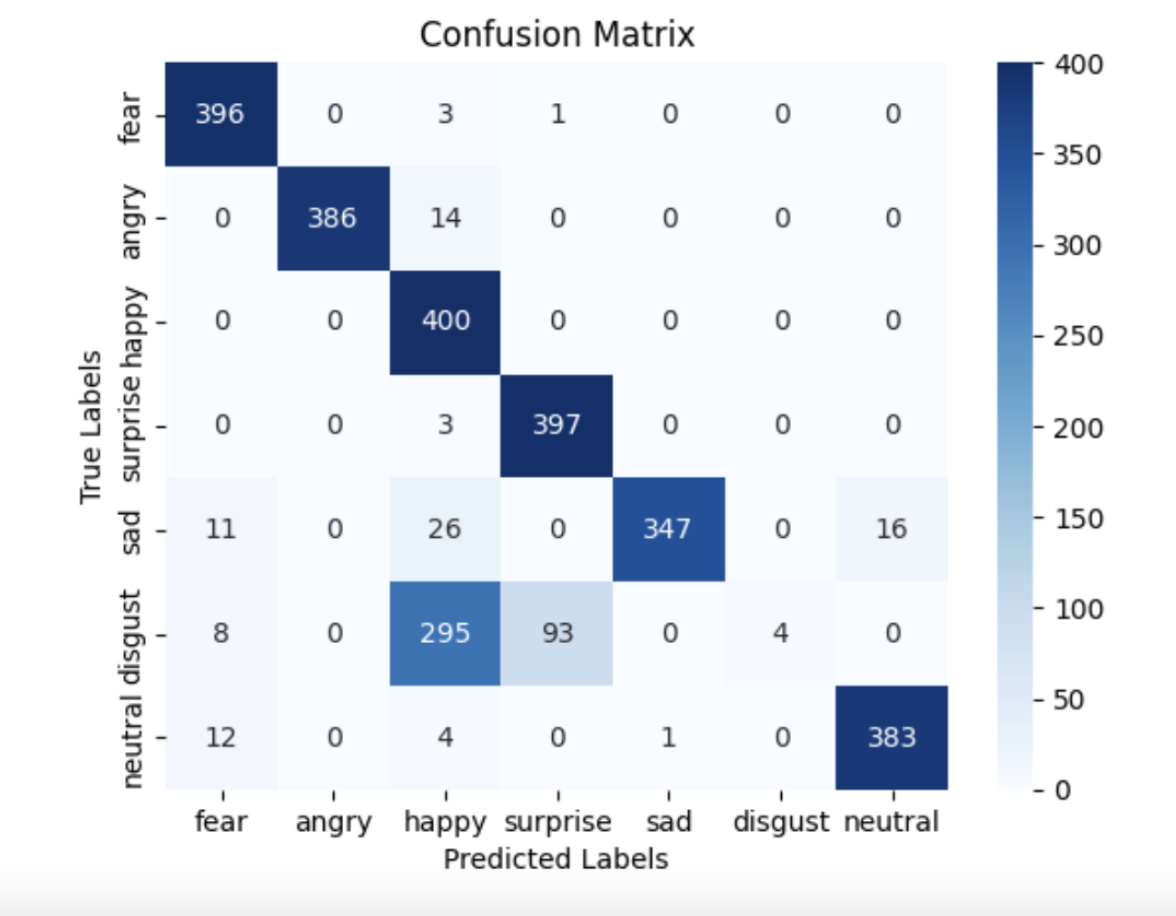
\includegraphics[width=1\linewidth]{ConfusionMatrix1.png}
\end{figure}
\newpage
\subsection{Performance of the Whisper-Large-V3 Model - With SAVEE Dataset}
\subsubsection{Final Evaluation Results}
\begin{figure}[H]
    \centering
    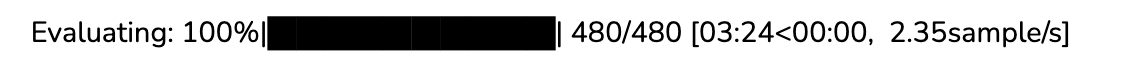
\includegraphics[width=1\linewidth]{521.png}
    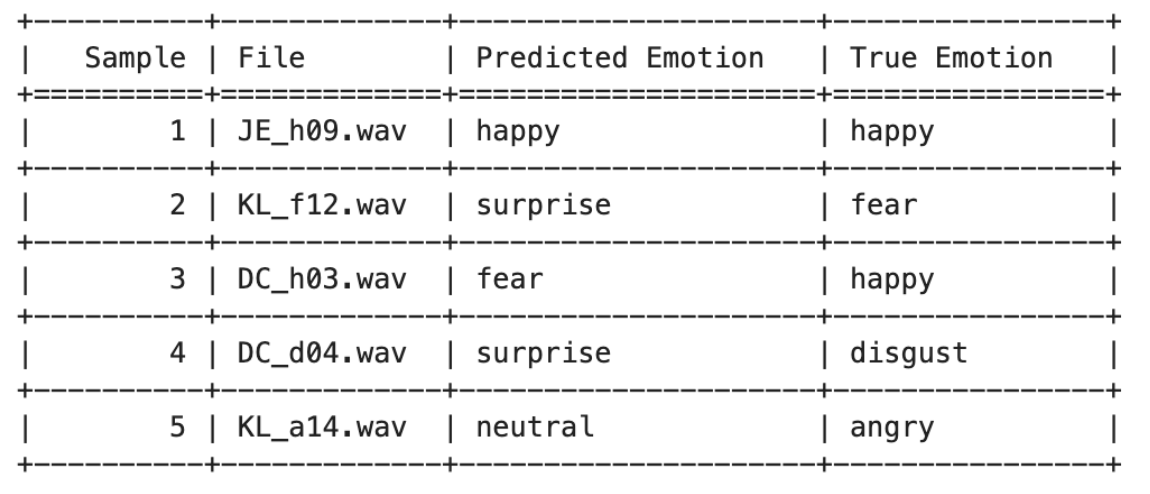
\includegraphics[width=1\linewidth]{522.png}
\end{figure}
\begin{figure}[H]
    \centering
    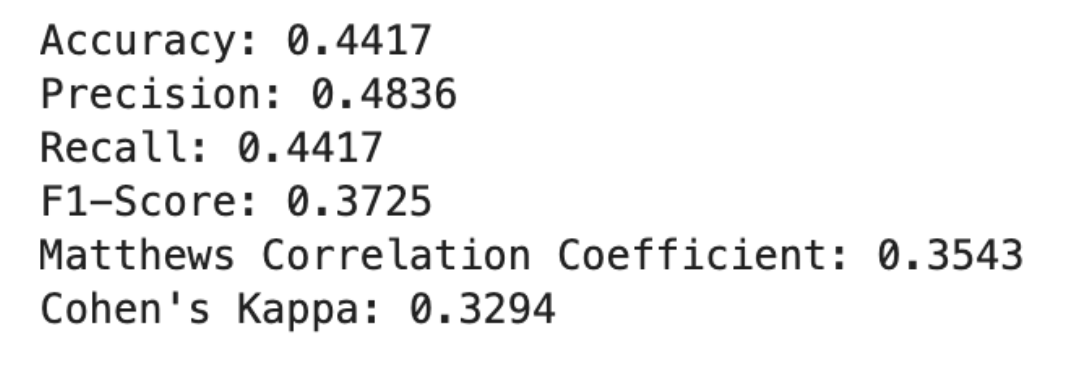
\includegraphics[width=1\linewidth]{523.png}
\end{figure}
\subsubsection{Classification Report}
\begin{figure}[H]
    \centering
    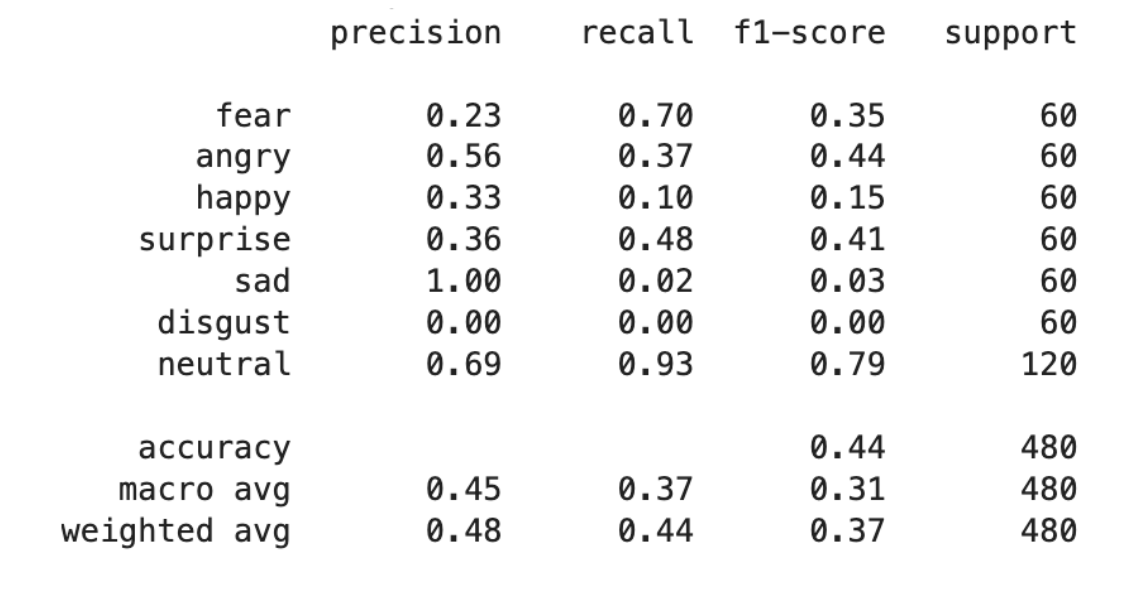
\includegraphics[width=1\linewidth]{545.png}
\end{figure}
\subsubsection{Confusion Matrix}
\begin{figure}[H]
    \centering
    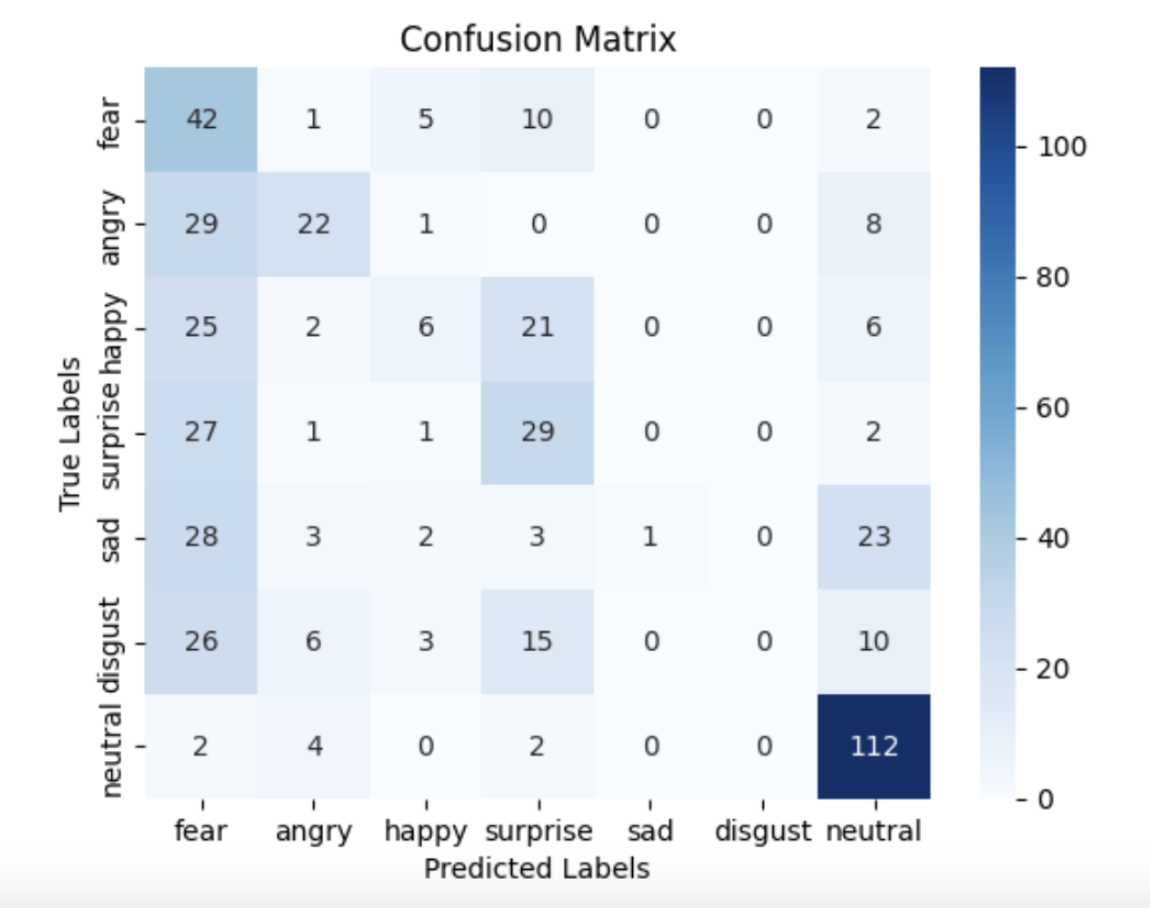
\includegraphics[width=1\linewidth]{525.png}
\end{figure}
\newpage
\subsection{Performance of the Wav2Vec 2.0 Model - with TESS Dataset}
\subsubsection{Final Evaluation Results}
\begin{figure}[H]
    \centering
    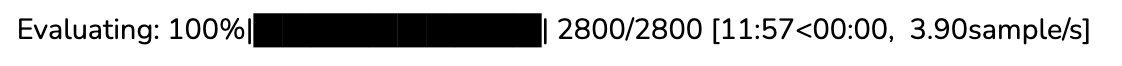
\includegraphics[width=1\linewidth]{5331.png}
    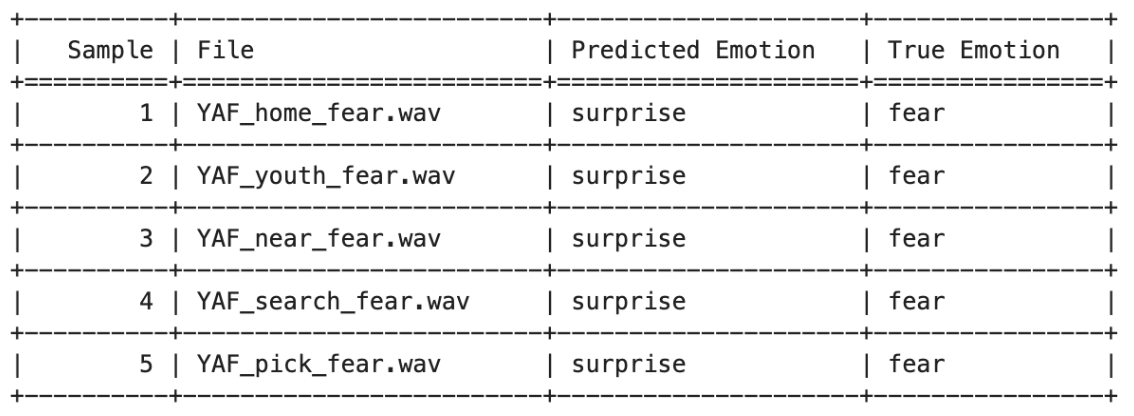
\includegraphics[width=1\linewidth]{5322.png}
\end{figure}
\begin{figure}[H]
    \centering
    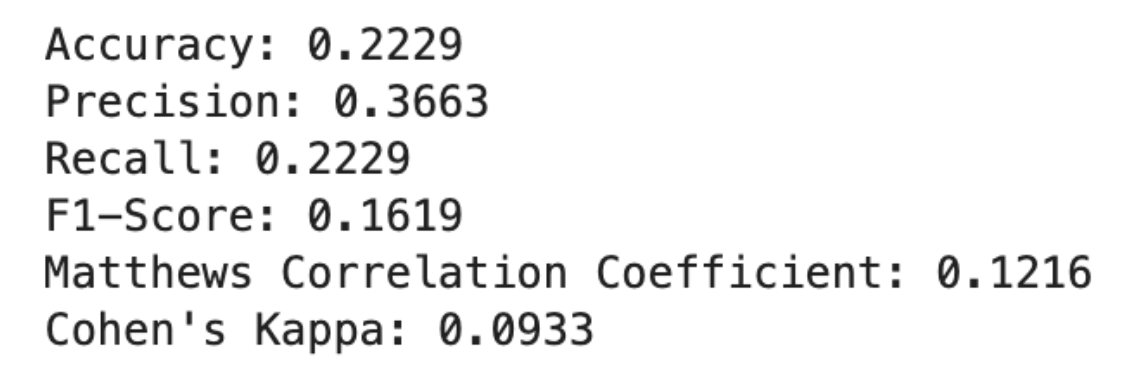
\includegraphics[width=1\linewidth]{5323.png}
\end{figure}
\subsubsection{Classification Report}
\begin{figure}[H]
    \centering
    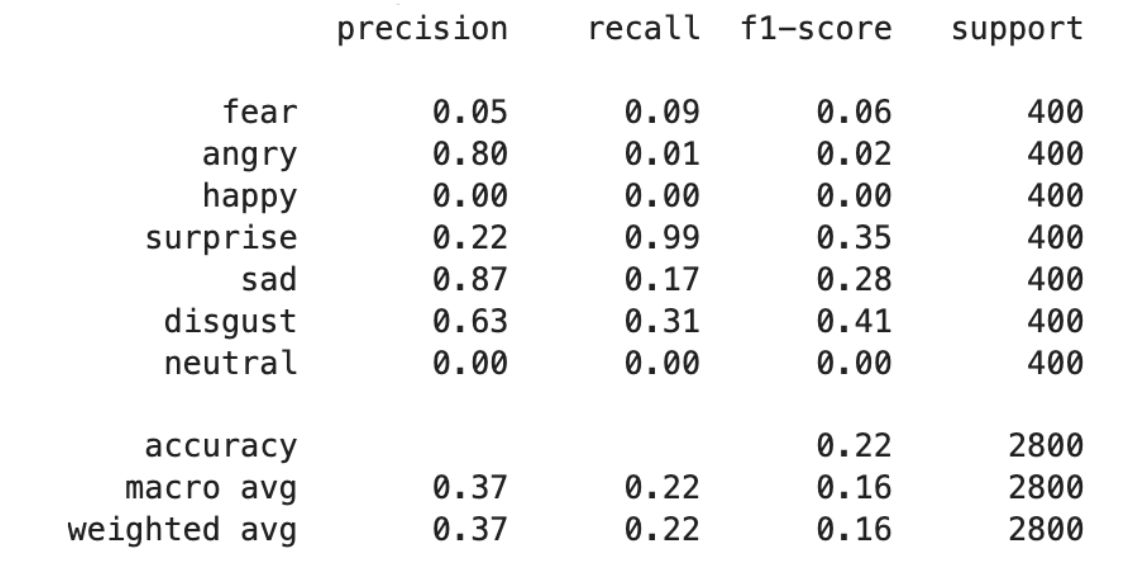
\includegraphics[width=1\linewidth]{5324.png}
\end{figure}
\subsubsection{Confusion Matrix}
\begin{figure}[H]
    \centering
    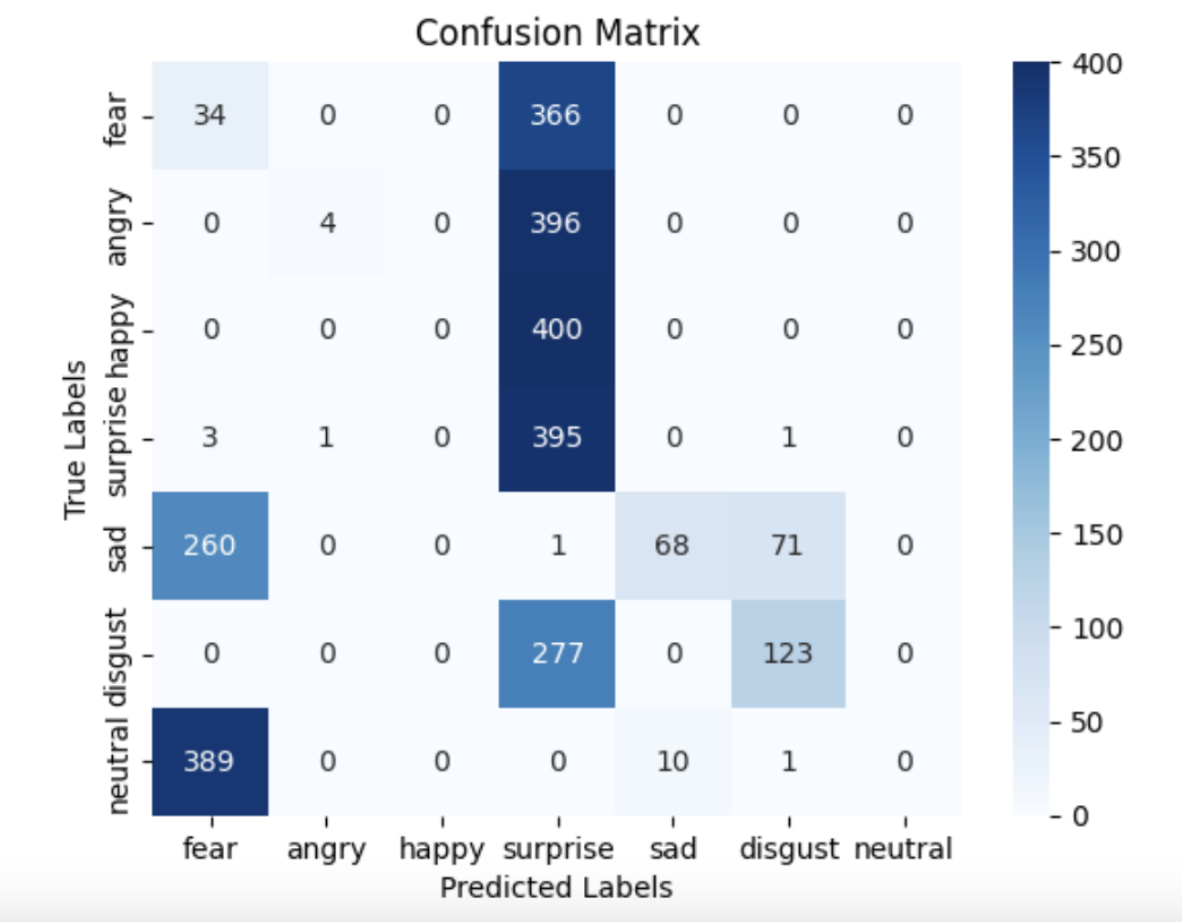
\includegraphics[width=1\linewidth]{5325.png}
\end{figure}
\newpage
\subsection{Performance of the Wav2Vec 2.0 Model - with SAVEE Dataset}
\subsubsection{Final Evaluation Results}
\begin{figure}[H]
    \centering
    
\includegraphics[width=1\linewidth]{5411.png}
    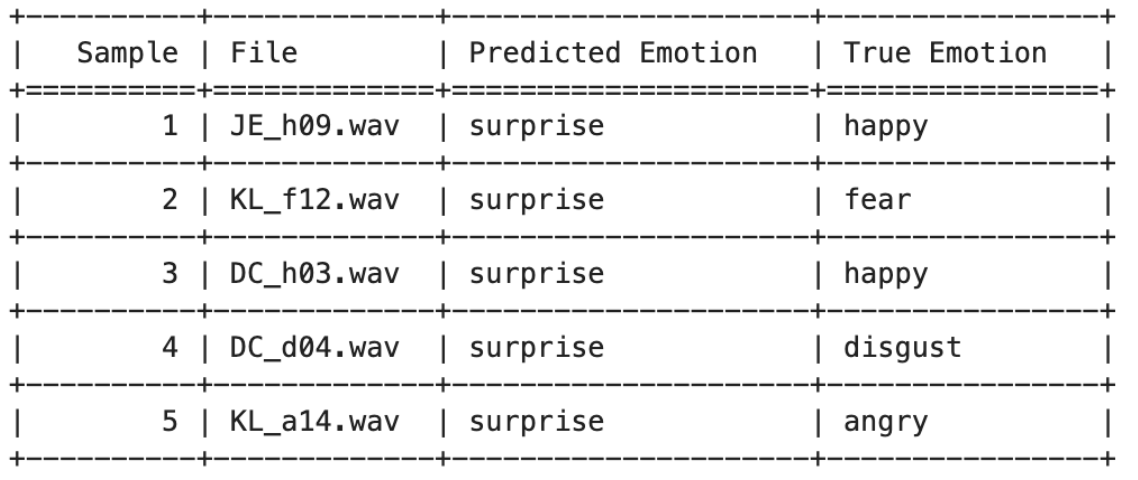
\includegraphics[width=1\linewidth]{5412.png}
\end{figure}
\begin{figure}[H]
    \centering
    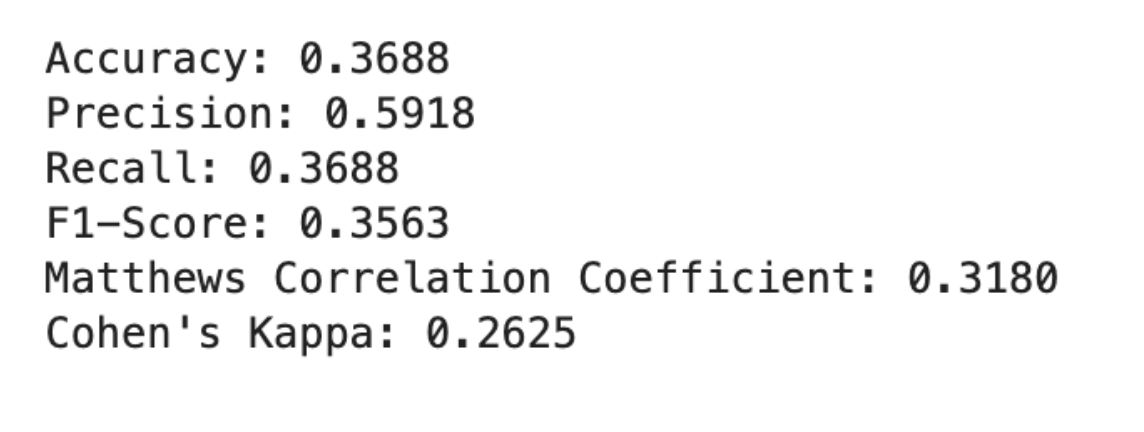
\includegraphics[width=1\linewidth]{5413.png}
\end{figure}
\subsubsection{Classification Report}
\begin{figure}[H]
    \centering
    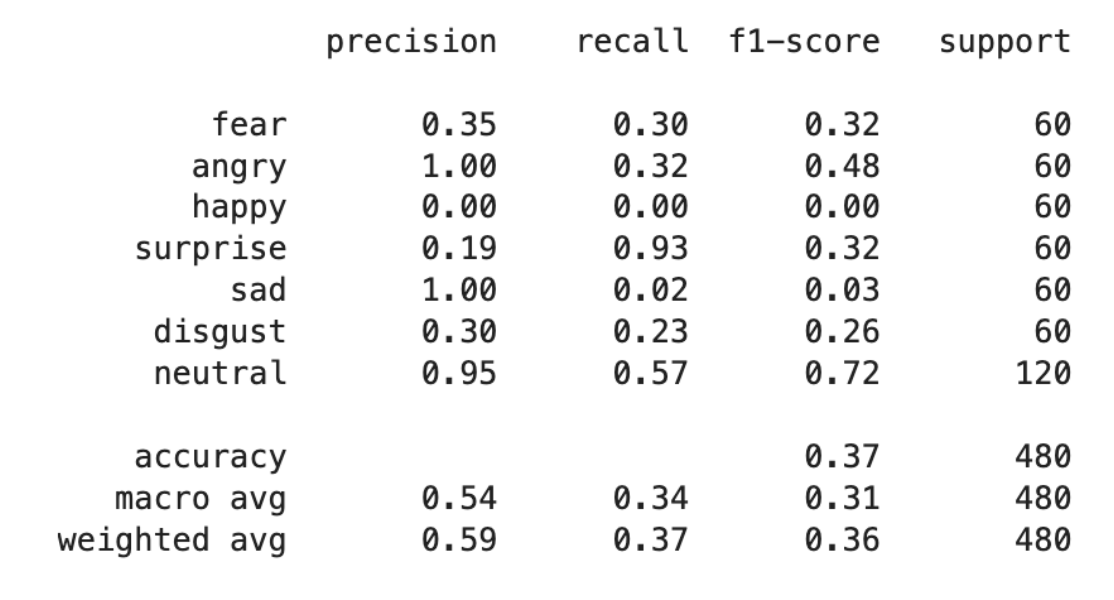
\includegraphics[width=1\linewidth]{5414.png}
\end{figure}
\subsubsection{Confusion Matrix}
\begin{figure}[H]
    \centering
    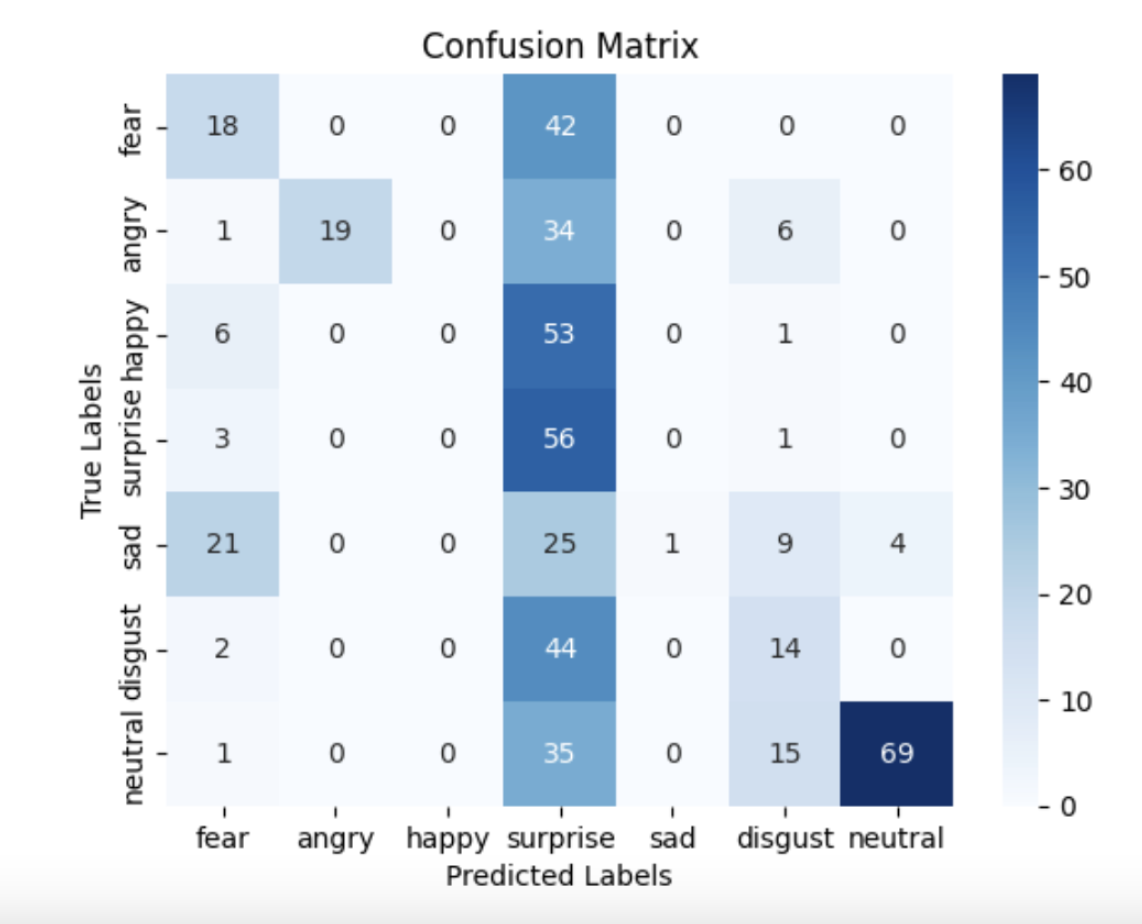
\includegraphics[width=1\linewidth]{5415.png}
\end{figure}
\newpage
\section{Comparative Study}
The performance of the Wav2Vec 2.0 and Whisper-Large-V3 models on the validation set highlights their effectiveness in speech recognition tasks, each offering unique strengths. The Whisper-Large-V3 model achieved a validation accuracy of 82.61%, whereas the Wav2Vec 2.0 model obtained a slightly lower accuracy of 22.29%. This suggests that while Whisper-Large-V3 demonstrates stronger overall performance, Wav2Vec 2.0 remains competitive, particularly in certain conditions where it may generalize better.
\begin{figure}[H]
    \centering
    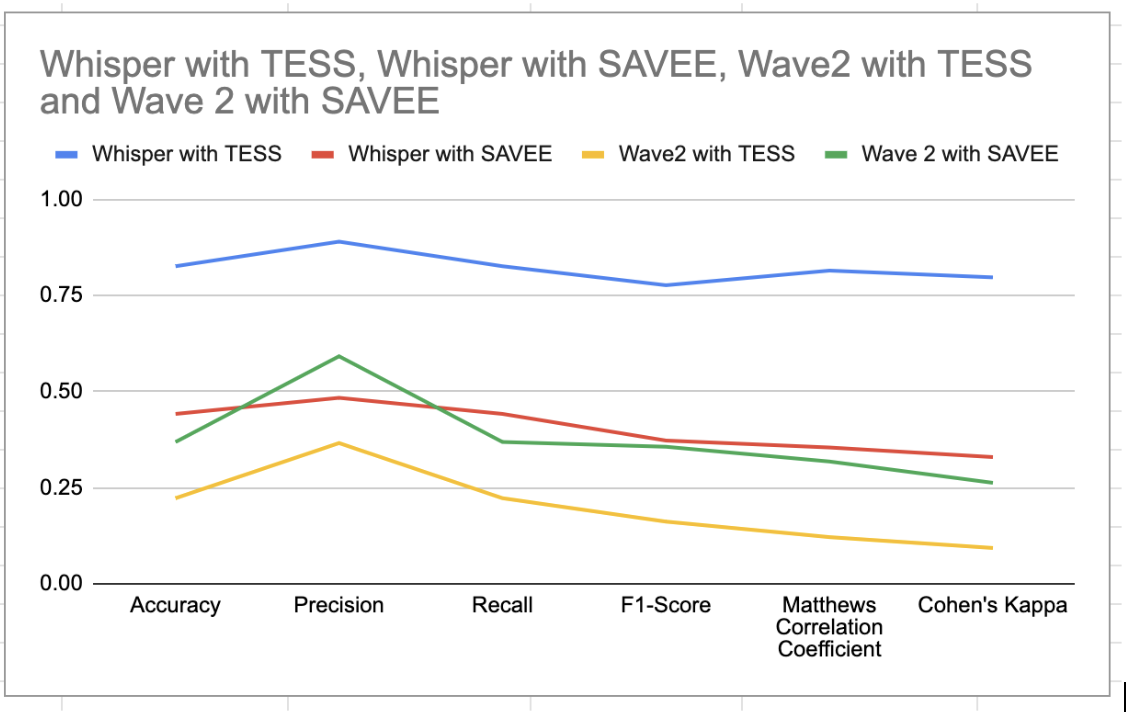
\includegraphics[width=1\linewidth]{611.png}
    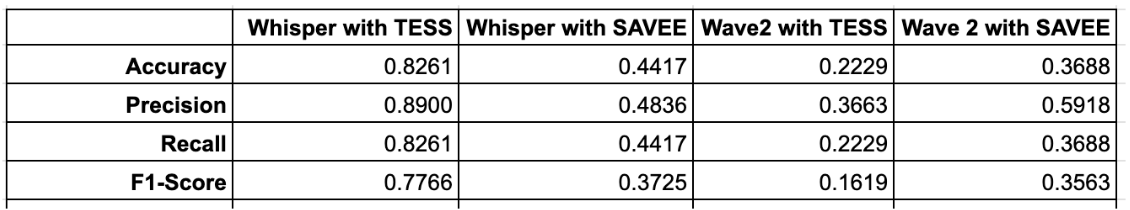
\includegraphics[width=1\linewidth]{612.png}
\end{figure}

Moving to the testing data, a direct comparison of these models under identical conditions provides deeper insights into their emotion recognition capabilities. As summarized in above table, both models exhibit high precision and recall across most emotional categories, yet key differences emerge:
\begin{itemize}


\item \textbf{Precision and Recall:} Whisper-Large-V3 consistently achieves higher precision across most emotions, especially excelling in categories like ‘Angry’, ‘Sad’ and ‘disgust’. Meanwhile, Wav2Vec 2.0 demonstrates higher recall for emotions like ‘Surprise’, indicating its ability to capture emotional variations more effectively.
\item \textbf{F1-Score:} Wav2Vec 2.0 struggles with precision in certain categories, leading to lower F1-scores for ‘Happy’ and ‘Angry’. Conversely, Whisper-Large-V3 maintains a balanced precision-recall tradeoff, resulting in higher overall F1-scores.
\item \textbf{Macro and Weighted Accuracy:} While one models perform well, Whisper-Large-V3 attains a macro accuracy of 83\%, whereas Wav2Vec 2.0 lags slightly at 22\%, further solidifying the superior performance of Whisper-Large-V3 in recognizing emotions with higher consistency.
\end{itemize}
\paragraph{}
These findings suggest that Whisper-Large-V3 may be better suited for speech emotion recognition (SER) tasks, particularly in scenarios demanding high precision and balanced recognition across different emotions. However, attributing this performance solely to its model architecture is complex. The disparities may also arise from variations in pretraining conditions, complicating the task of isolating whether the advantage stems from the inherent architecture or pre-training methodology.
\paragraph{}
The Whisper-Large-V3 model benefits from extensive training on diverse multilingual datasets, enabling it to handle varied linguistic nuances effectively. On the other hand, Wav2Vec 2.0, trained on a more domain-specific dataset, might exhibit strengths in scenarios where fine-grained recall is essential. This underscores the challenges in evaluating self-supervised learning models, where both architecture and pretraining conditions significantly influence performance.
\paragraph{}
Thus, while architecture plays a crucial role in determining model effectiveness, the pretraining dataset and its alignment with the target task remain equally pivotal in achieving optimal results for SER applications.

\end{itemize}
\newpage
\section{Conclusion}
This study aimed to compare the performance of the Wav2Vec 2.0 and Whisper-Large-V3 models in recognizing emotions from speech within an End-to-End SER system. Our findings highlight that Whisper-Large-V3 consistently outperforms Wav2Vec 2.0 across multiple evaluation metrics, achieving higher accuracy, precision, and F1-scores, particularly in recognizing emotions such as ‘Happy,’ ‘Neutral,’ and ‘Disgust.’ Conversely, Wav2Vec 2.0 demonstrated strengths in recall, particularly for emotions like ‘Surprise.’
\paragraph{}
The results suggest that Whisper-Large-V3 is better suited for SER tasks requiring high precision and balanced emotion classification. However, the role of pretraining conditions cannot be overlooked. The superior performance of Whisper-Large-V3 may be attributed not only to its architecture but also to the diversity of its pretraining data, which enables better generalization. In contrast, Wav2Vec 2.0, with its domain-specific pretraining, exhibits strengths in certain contexts but struggles with overall precision.
\paragraph{}
Future work should focus on isolating the effects of model architecture and pretraining conditions by conducting controlled experiments where both models are trained on identical datasets. Additionally, expanding the evaluation to include diverse linguistic and cultural contexts will provide a more comprehensive understanding of each model’s strengths and limitations. These insights will be crucial in optimizing SER systems for real-world applications.
\newpage
\section{Code Repository}
\href{https://github.com/IITJ-Projects/M23CSA545_PA1.git}{ GitHub Repository}
\addcontentsline{toc}{section}{References}
%\addbibresource{references.bib}
%\printbibliography[heading=bibintoc, title={References}]
\begin{thebibliography}{9}
    \bibitem{example} \href{https://www.kaggle.com/code/swish9/audio-emotion-recognition-with-pytorch}{Audio Emotion Recognition with PyTorch}
    \bibitem{example2} \href{https://www.kaggle.com/code/shivamburnwal/speech-emotion-recognition}{Speech Emotion Recognition}
    \bibitem{example3} \href{https://www.kaggle.com/code/mostafaabdlhamed/speech-emotion-recognition-97-25-accuracy}{ Speech emotion recognition 97.25\% accuracy}
    \bibitem{example4} \href{https://www.kaggle.com/datasets/dmitrybabko/speech-emotion-recognition-en}{ Speech Emotion Recognition (en)}
    \bibitem{documentation} \href{https://www.overleaf.com/}{ Latex Documentation - Overleaf}
\end{thebibliography}
\end{document}
